%%%%%%%%%%%%%%%%%%%%%%%%%%%%%%%%%%%%%%
\chapter{Studies on track reconstruction problems}\label{app:tobtec}
%%%%%%%%%%%%%%%%%%%%%%%%%%%%%%%%%%%%%%

A scan of the displays of all the events in 8\TeV data with $\mWH >$ 1.6\TeV passing all the selection criteria for the $\ell\Pgn\bbbar$ final state (Table~\ref{tab:cutsummaryWH})
reported that presence of two events characterized by a rare type of background.
This background arises when particles back scatter from the calorimeter to the tracker, causing non-prompt real tracking hits.
Although this behavior occurs everywhere in the detector, the track reconstruction is particularly affected by it in the transition region between the barrel (TOB) and endcap (TEC) of the silicon tracker, namely, in the pseudorapidity range 1~$<|\eta|<$~1.5 (Fig.~\ref{fig:TrackerLayout}).
In this region, the track reconstruction algorithm considers these hits to build track candidates, such that many fake (displaced) tracks are associated to the selected H-jet candidate.
%This noise arises from an anomalous behaviour of the tracking algorithm in the transition region between the barrel (TOB) and endcap (TEC) regions of the silicon tracker,
%namely, in the pseudorapidity range 1~$<|\eta|<$~1.5 (Fig.~\ref{fig:TrackerLayout}). As a consequence, many fake (displaced) tracks are associated to the selected H-jet candidate.
Figure~\ref{fig:BadEventData} shows the event display of one of the two events
affected by this problem, while Figure~\ref{fig:BadEventMC} shows the same feature in simulation.

In order to reject this background, it is common in CMS analyses to apply a standard filtering algorithm that discards the event if 
there is an anomalous amount of tracks that have been seeded in the TOB-TEC transition region.
The efficiency of this filter on signal events is about 97\% independently on the H-jet \pt.

\begin{figure}[!htb]
\centering
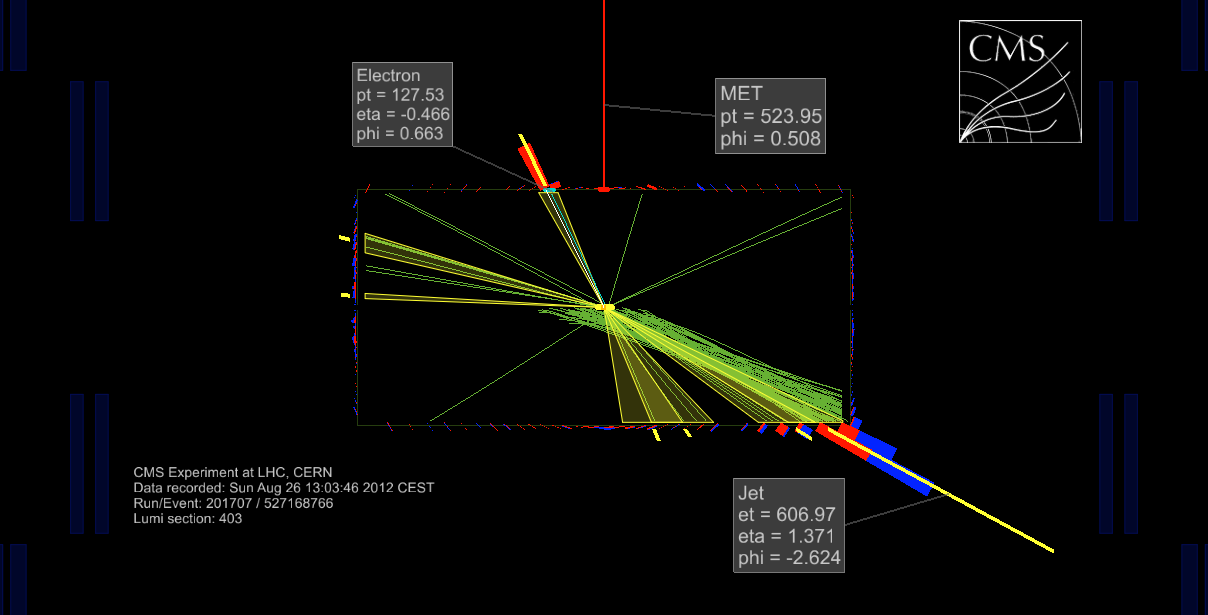
\includegraphics[width=0.75\textwidth]{Appendix/Figures/SingleEleC_Run201707_Event527168766_Lumi403_badEvent.png}
\caption{Display of one typical anomalous event found in data recorded by the CMS experiment. 
Many fake and displaced tracks are reconstructed creating a bias in the jet reconstruction.
Only tracks with \pt larger than 2\GeV are shown.}
\label{fig:BadEventData}
\end{figure}

\begin{figure}[!htb]
\centering
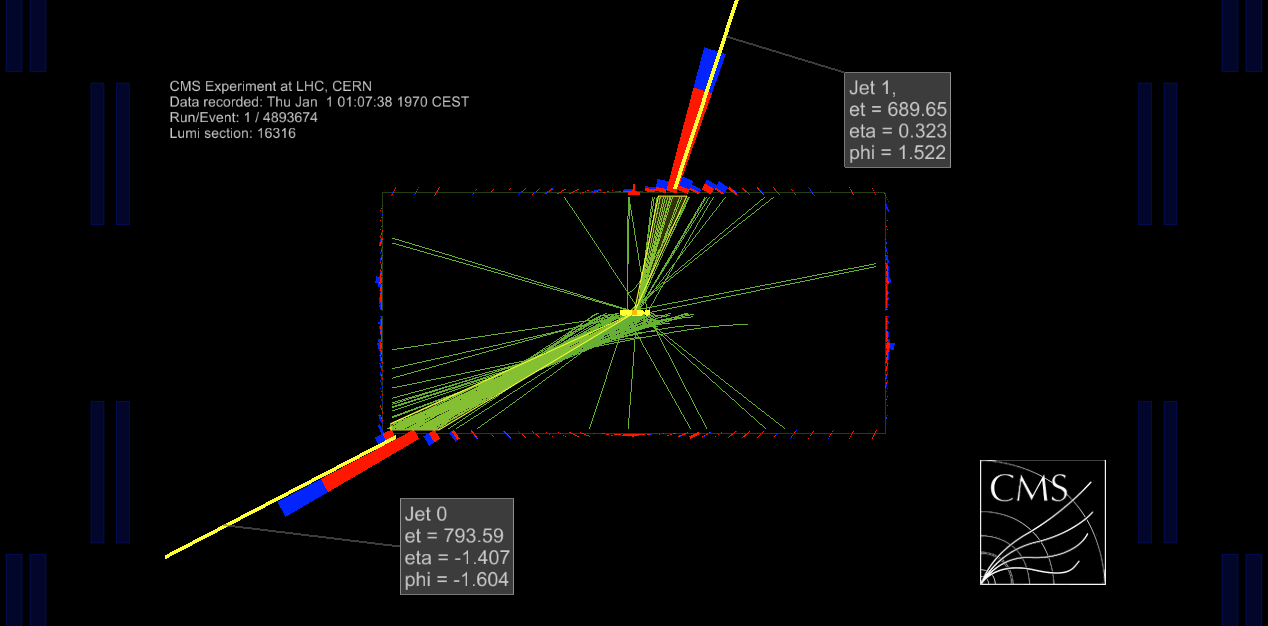
\includegraphics[width=0.75\textwidth]{Appendix/Figures/MCevent-with-tobtec.png}
\caption{Display of one typical anomalous event in simulation.
Only tracks with \pt larger than 2\GeV are shown.}
\label{fig:BadEventMC}
\end{figure}

However, further checks performed on the anomalous events showed that after applying the standard filter 
residual noise can still be identified in the problematic $\eta$ region. Therefore, it has been decided for the analysis described in this work to
apply an additional requirement on the $\eta$ of the selected H-jet candidate (Section~\ref{subsec:jetsreco}).
In particular, CA8 jets are rejected if their pseudorapidity falls in the problematic region 1~$<|\eta|<$~1.8.
As described in the following, the choice for this fiducial cut is motivated by the disagreement between data and simulation in the rate
at which this background occurs.

The efficiency of the standard filter is studied as a function of the H-jet \pt and $\eta$ in a dijet sample with high statistics in both data and simulation.
%The datasets used for these studies are summarized in Table~\ref{data-dijet}. Events are selected if one of the following trigger has fired: 
%HLT\_PFJet320, HLT\_PFHT650, HLT\_PFNoPUHT650. The performance of the filters in simulation has been studied 
%using the QCD MC samples listed in Table~\ref{mc-bkg-dijet}.
The sample is selected requiring at least two jets, with $\pt > 400\GeV$ for the leading jet and $\pt > 80\GeV$ for the sub-leading one.
At least one of the jets has to be b tagged using the same combined b-tagging algorithm as for the main analysis selection, representing thus the H-jet candidate.
The jet that fails the b tagging is required to have low pruned mass ($\mJ < 40\GeV$).

Figure~\ref{fig:hbbjeteta} shows the effect of the filter on the jet $\eta$ distribution comparing data, simulated signal and QCD background:
the signal distribution is rather unaffected while data and QCD background distributions show a reduction of events in the problematic $\eta$ region after applying the filter, as expected.

\begin{figure}[!htb]
\centering
\subfigure[]{\label{fig:hbbjeteta_a}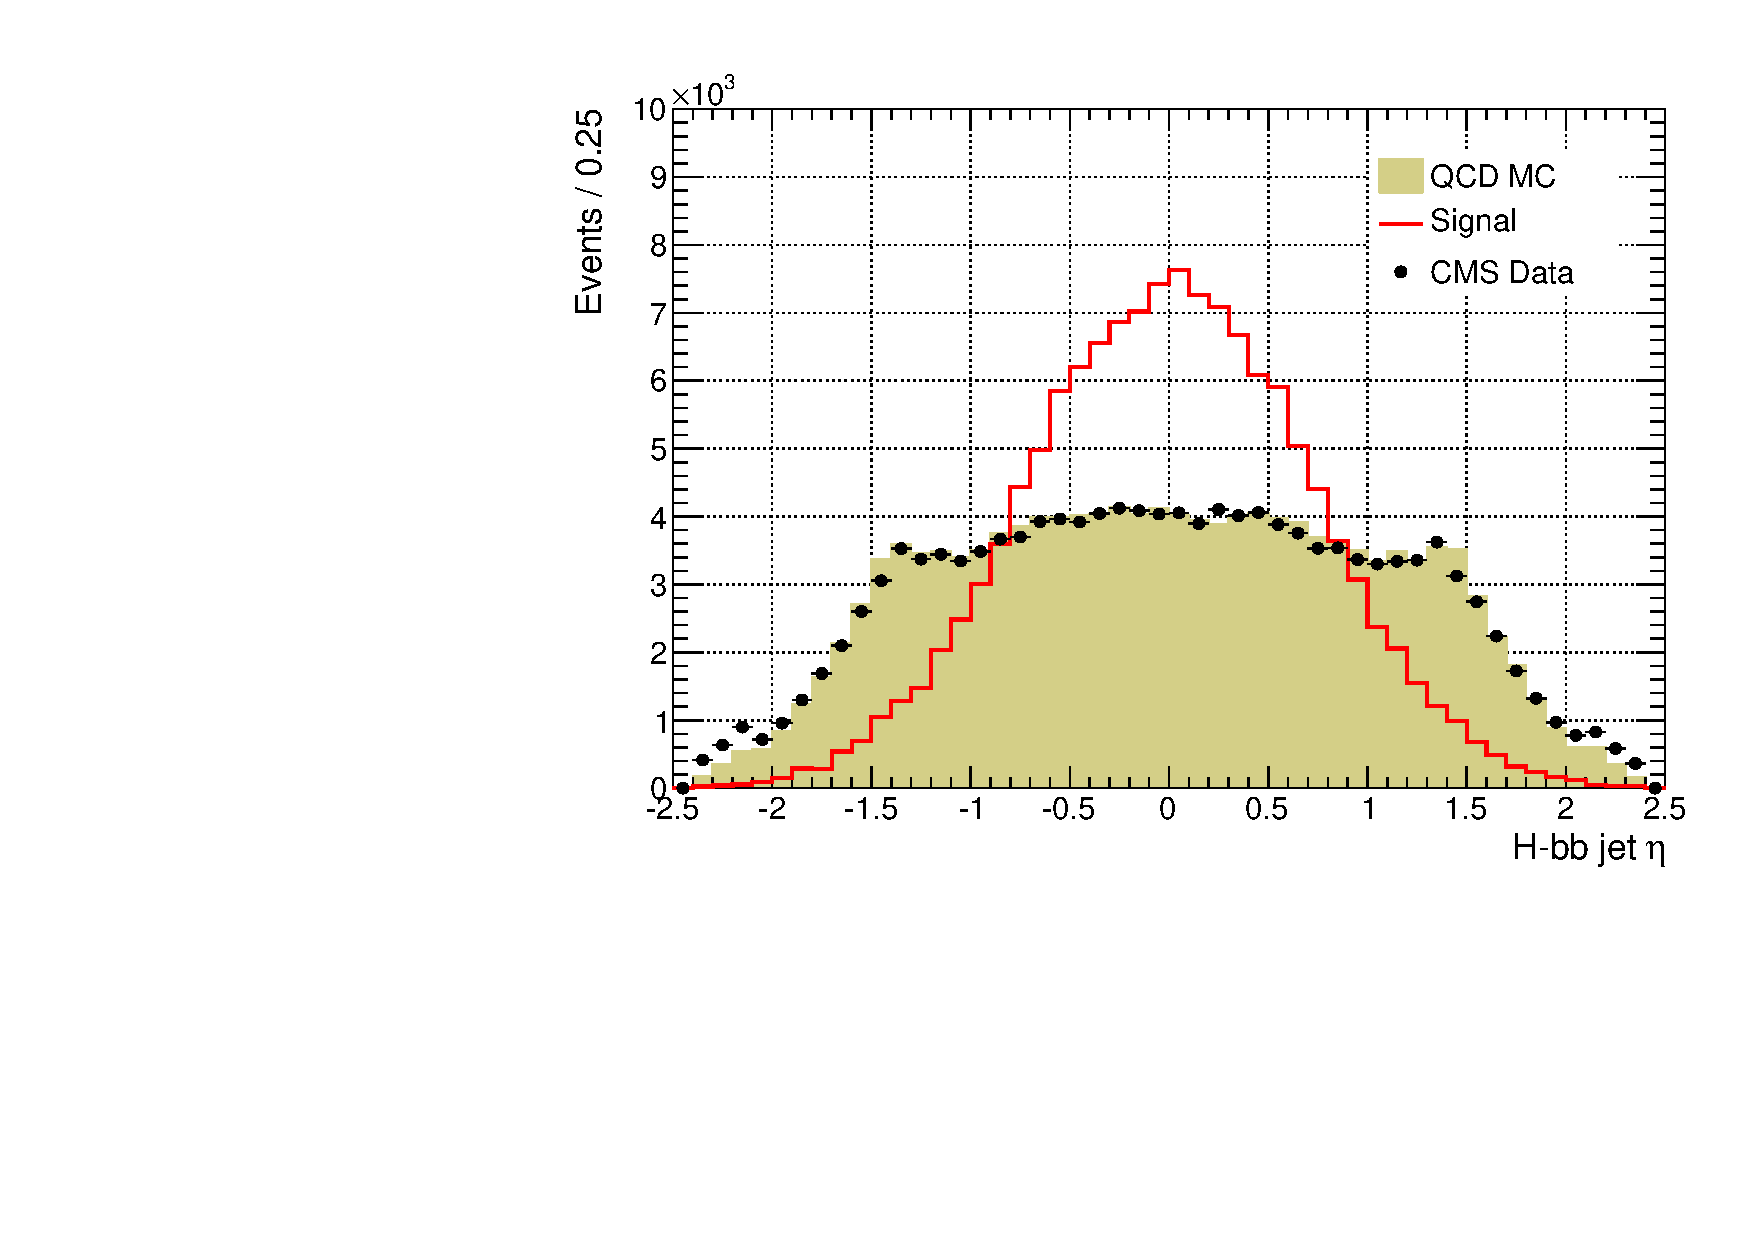
\includegraphics[width=0.45\textwidth]{Appendix/Figures/hbbjet-eta-nofilters.pdf}}
\subfigure[]{\label{fig:hbbjeteta_b}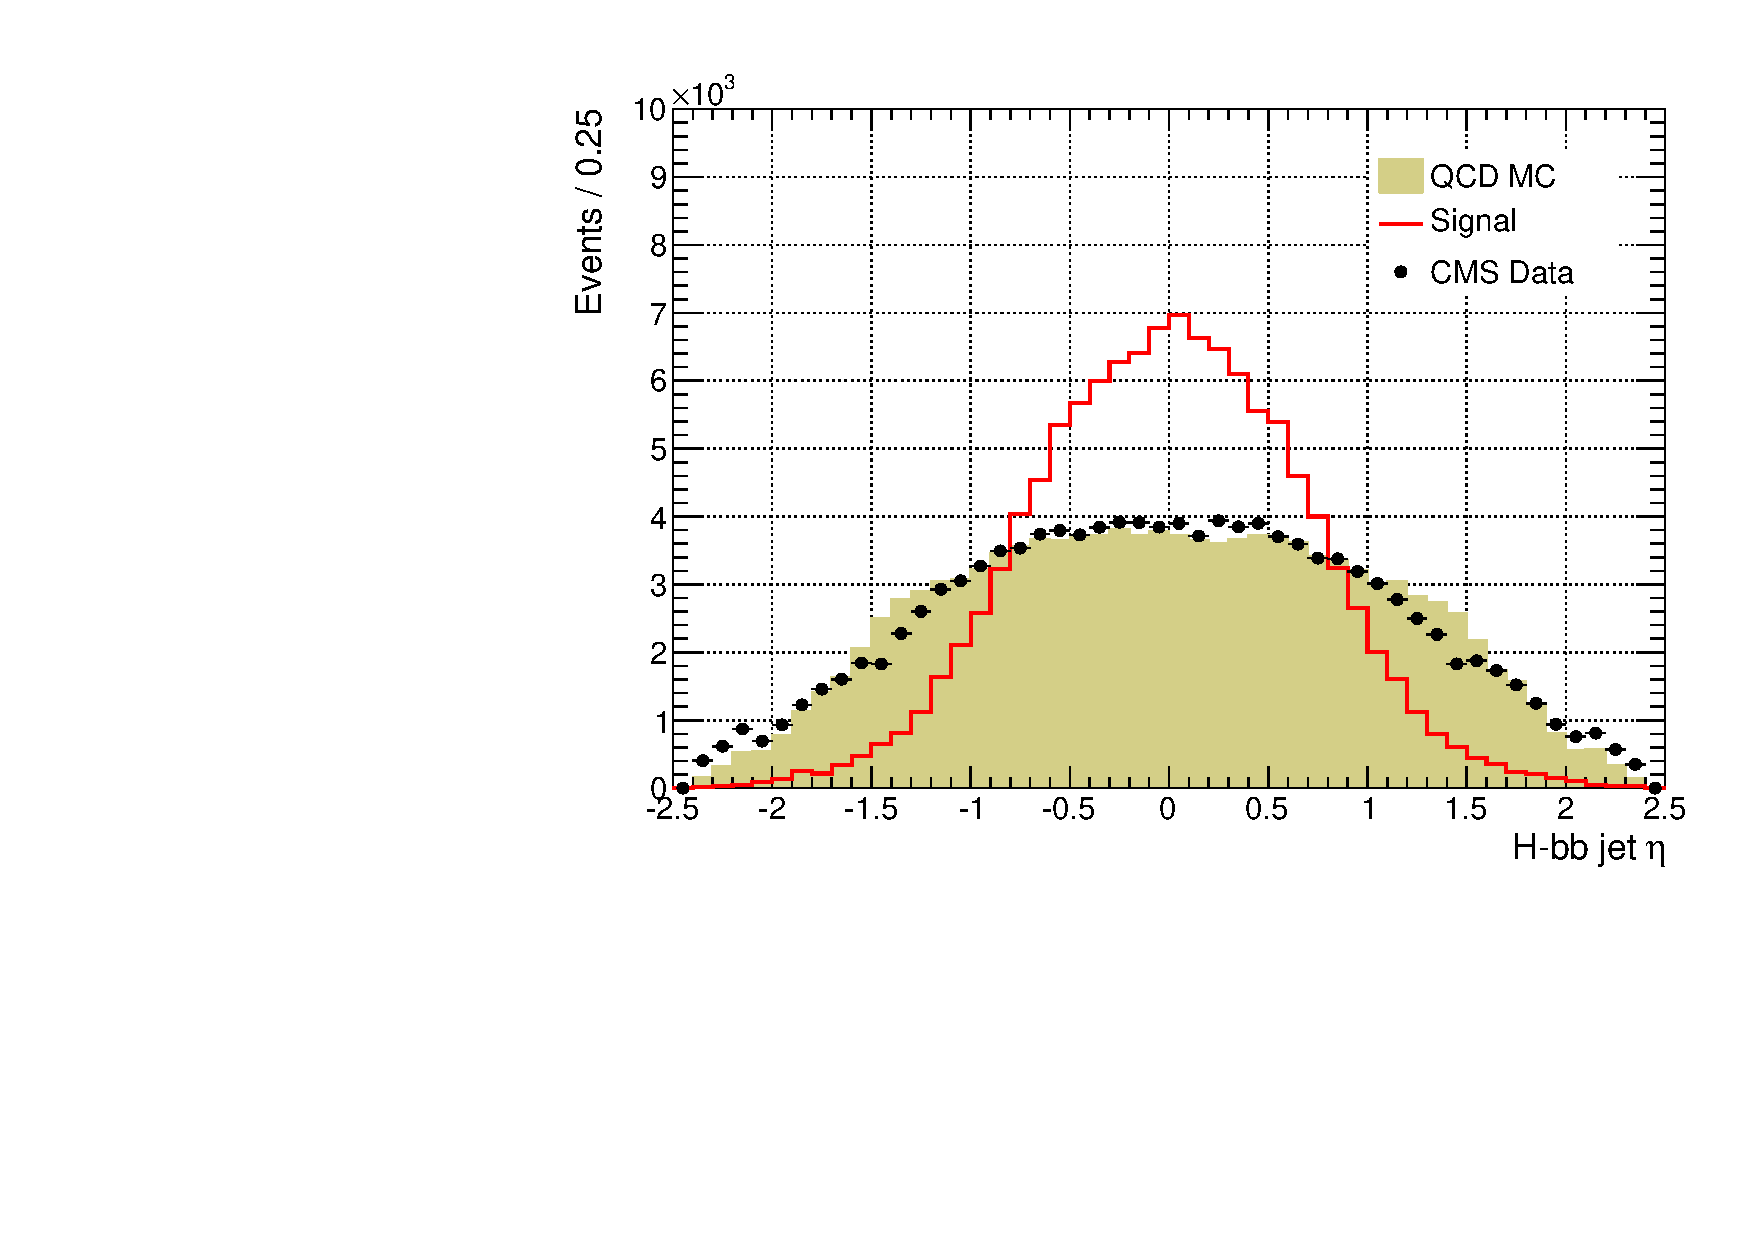
\includegraphics[width=0.45\textwidth]{Appendix/Figures/hbbjet-eta-tobtecfilter.pdf}}
\caption{Comparison of the H-jet $\eta$ distributions for data, and simulated signal and QCD background before (a) and after (b) applying the
tracking noise filter. Signal jets are mostly central in the detector.}
\label{fig:hbbjeteta}
\end{figure}

Figure~\ref{fig:eff-pt-filters-eta1} shows the filter efficiency on data and simulated signal and QCD background as a function 
of the H-jet candidate \pt for different jet $\eta$ regions.
A little dependence of the filter efficiency with the jet \pt is observed in the regions $0 < |\eta| < 1$ and $1.0 < |\eta| < 1.5$, 
while in the forward region $1.5 < |\eta| < 2.4$ the efficiency decreases with the jet \pt. 
The performance of the filter in the different $\eta$ regions is summarized in Figure~\ref{fig:eff-filters-eta_a}.
A large discrepancy between data and simulation is found in the pseudorapidity region $1.0 < |\eta| < 1.8$, 
where the simulation does not sufficiently well describe the full material budget of the tracking detector.
The same studies are also performed removing the b-tagging requirement. The filter efficiency as a function of the leading 
jet $\eta$ for this case is shown in Fig.~\ref{fig:eff-filters-eta_b}, for both data and simulation.
The increase in efficiency compared to what was obtained with b tagging shows that 
the b-tagging requirement enriches the samples with events characterized by this noise up to 30\%, making this analysis systematically prone to it.

\begin{figure}[!htb]
\centering
\subfigure[]{\label{fig:eff-pt-filters-eta1_a}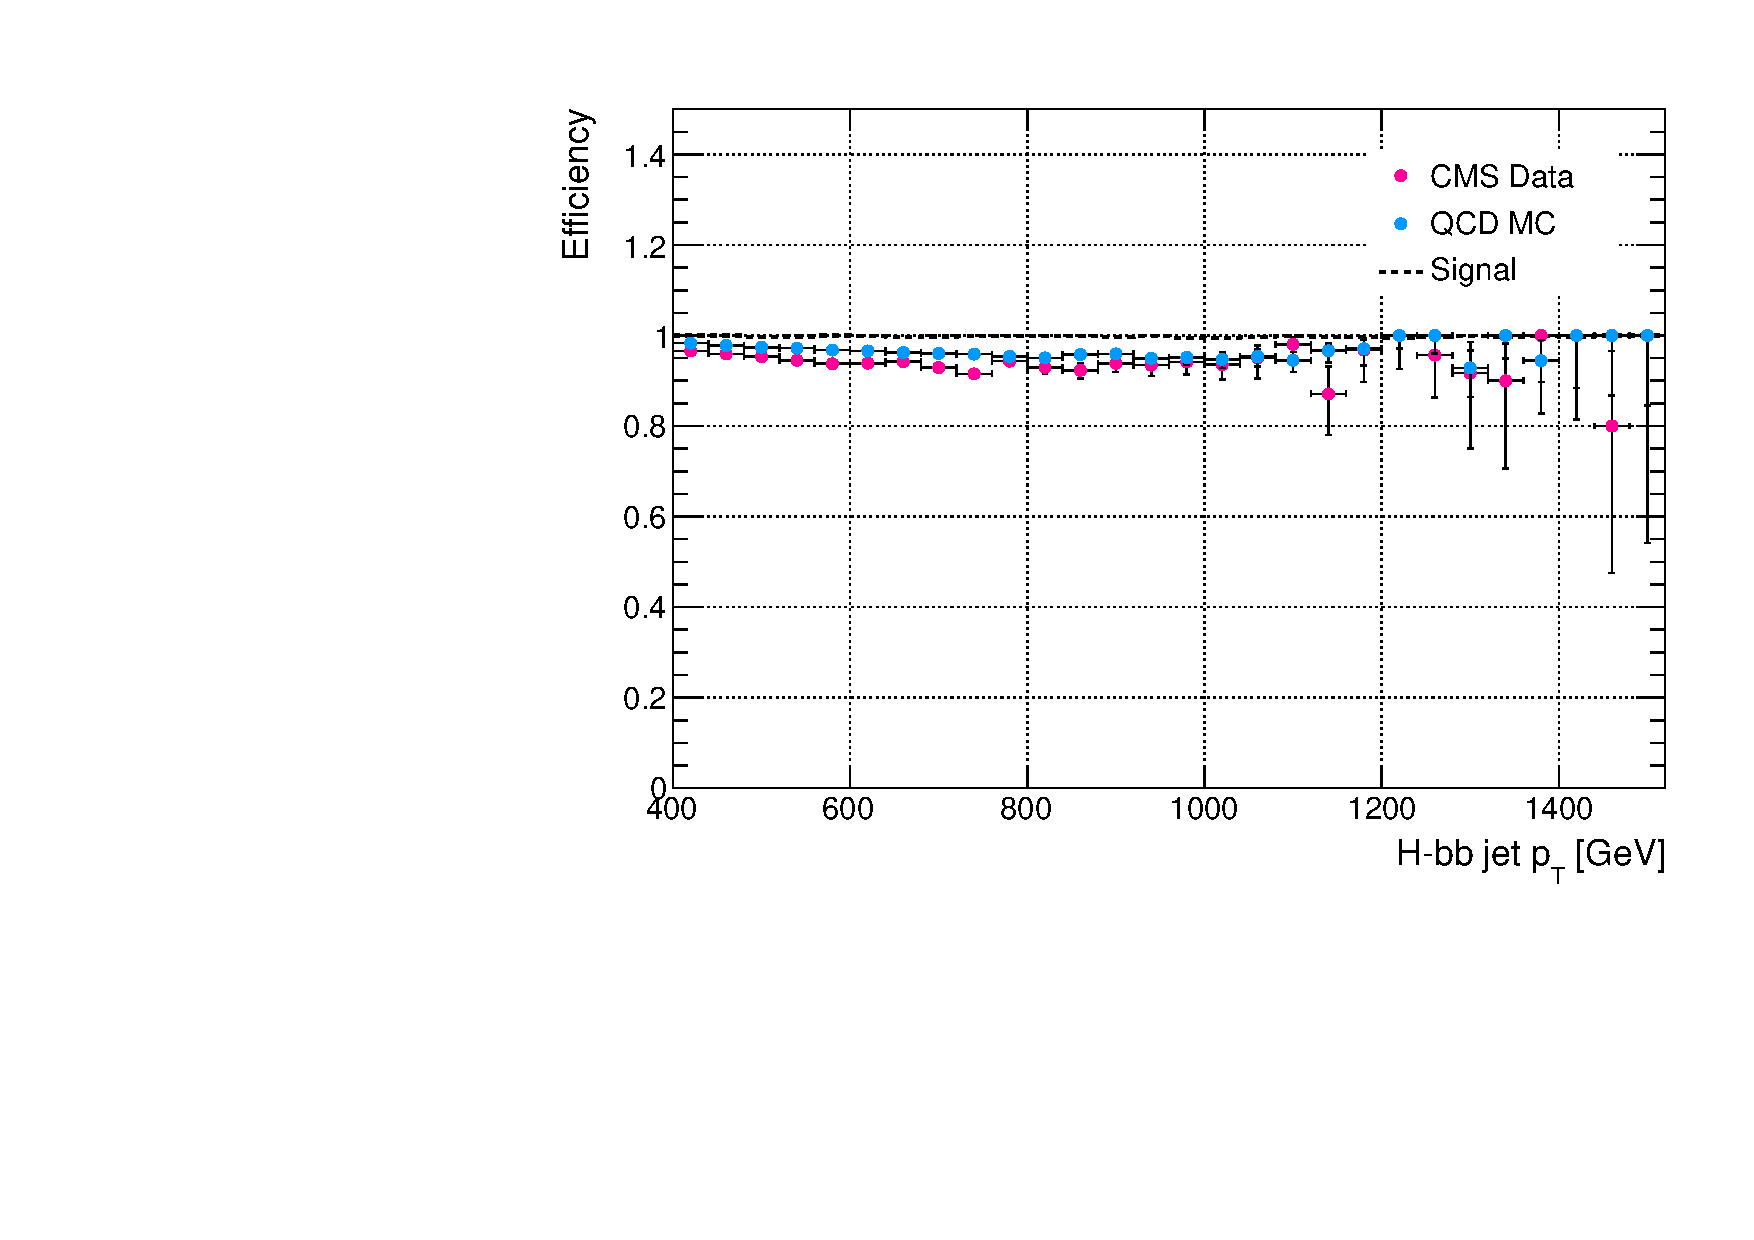
\includegraphics[width=0.3\textwidth]{Appendix/Figures/eff-pt-tobtecfilter-eta_0_1.pdf}}
\subfigure[]{\label{fig:eff-pt-filters-eta1_b}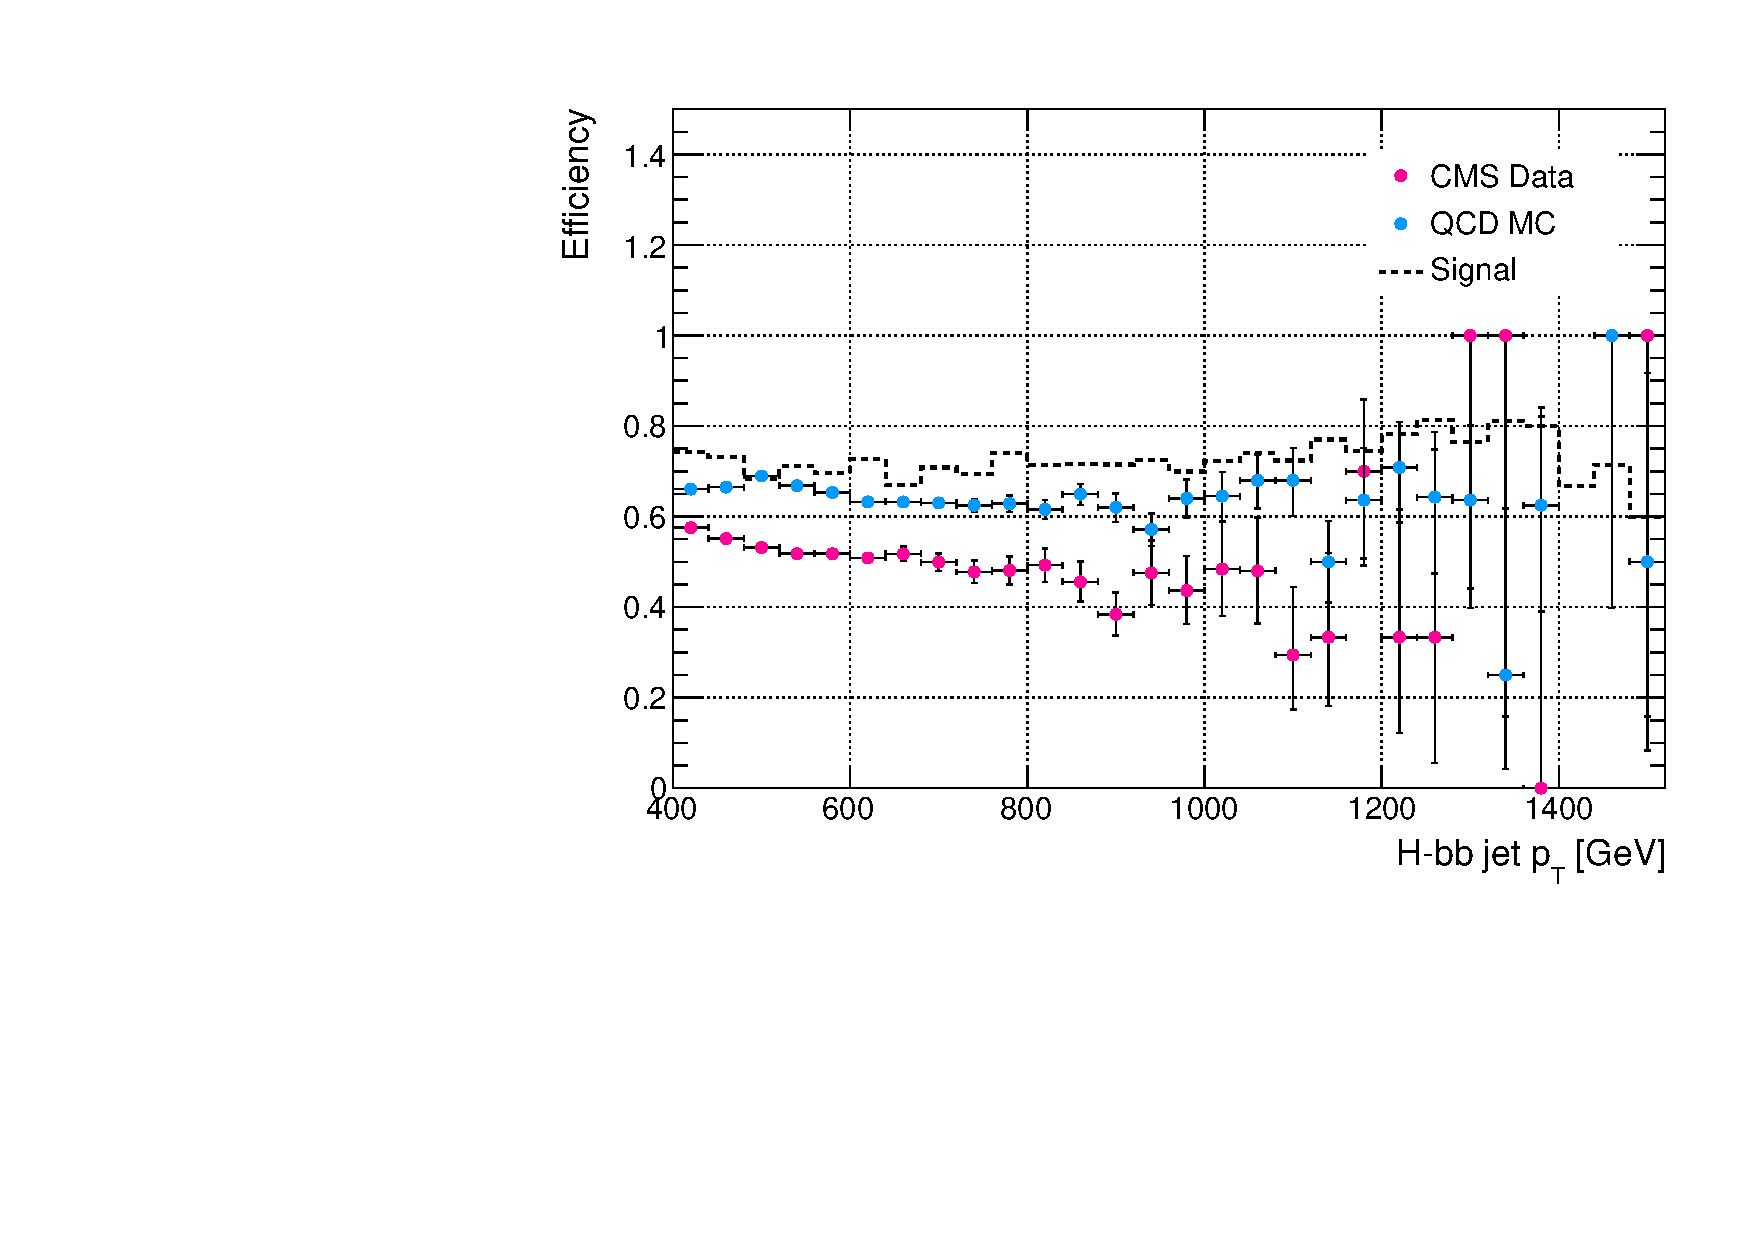
\includegraphics[width=0.3\textwidth]{Appendix/Figures/eff-pt-combinedfilters-eta_1_1p5.pdf}}
\subfigure[]{\label{fig:eff-pt-filters-eta1_c}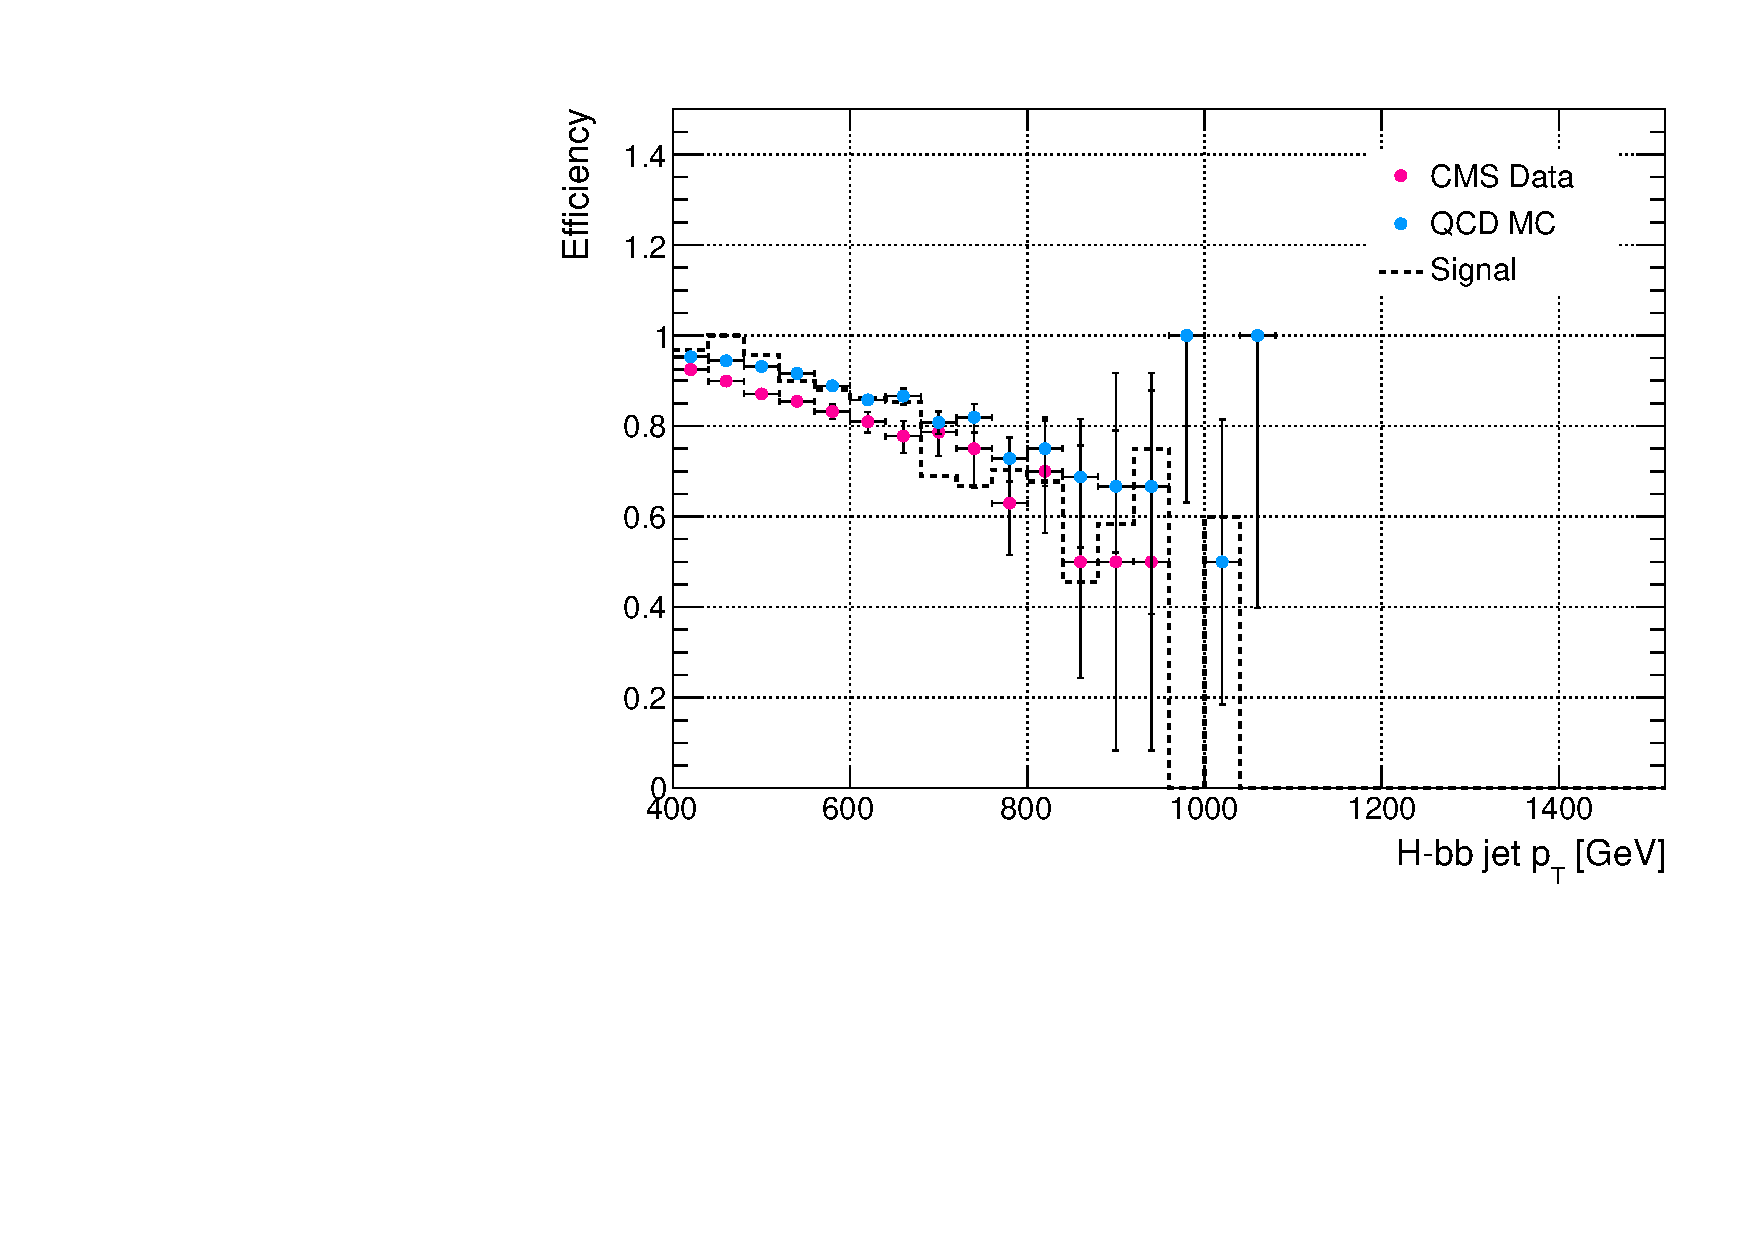
\includegraphics[width=0.3\textwidth]{Appendix/Figures/eff-pt-tobtecfilter-eta_1p5_2p4.pdf}}
\caption{Efficiency of the tracking noise filter as a function of the H-jet \pt for data, and simulated signal and QCD background
for jets reconstructed in the pseudorapidty regions $0 < |\eta| < 1$ (a), $1.0 < |\eta| < 1.5$ (b), and $1.5 < |\eta| < 2.4$ (c).}
\label{fig:eff-pt-filters-eta1}
\end{figure}

\begin{figure}[!htb]
\centering
\subfigure[]{\label{fig:eff-filters-eta_a}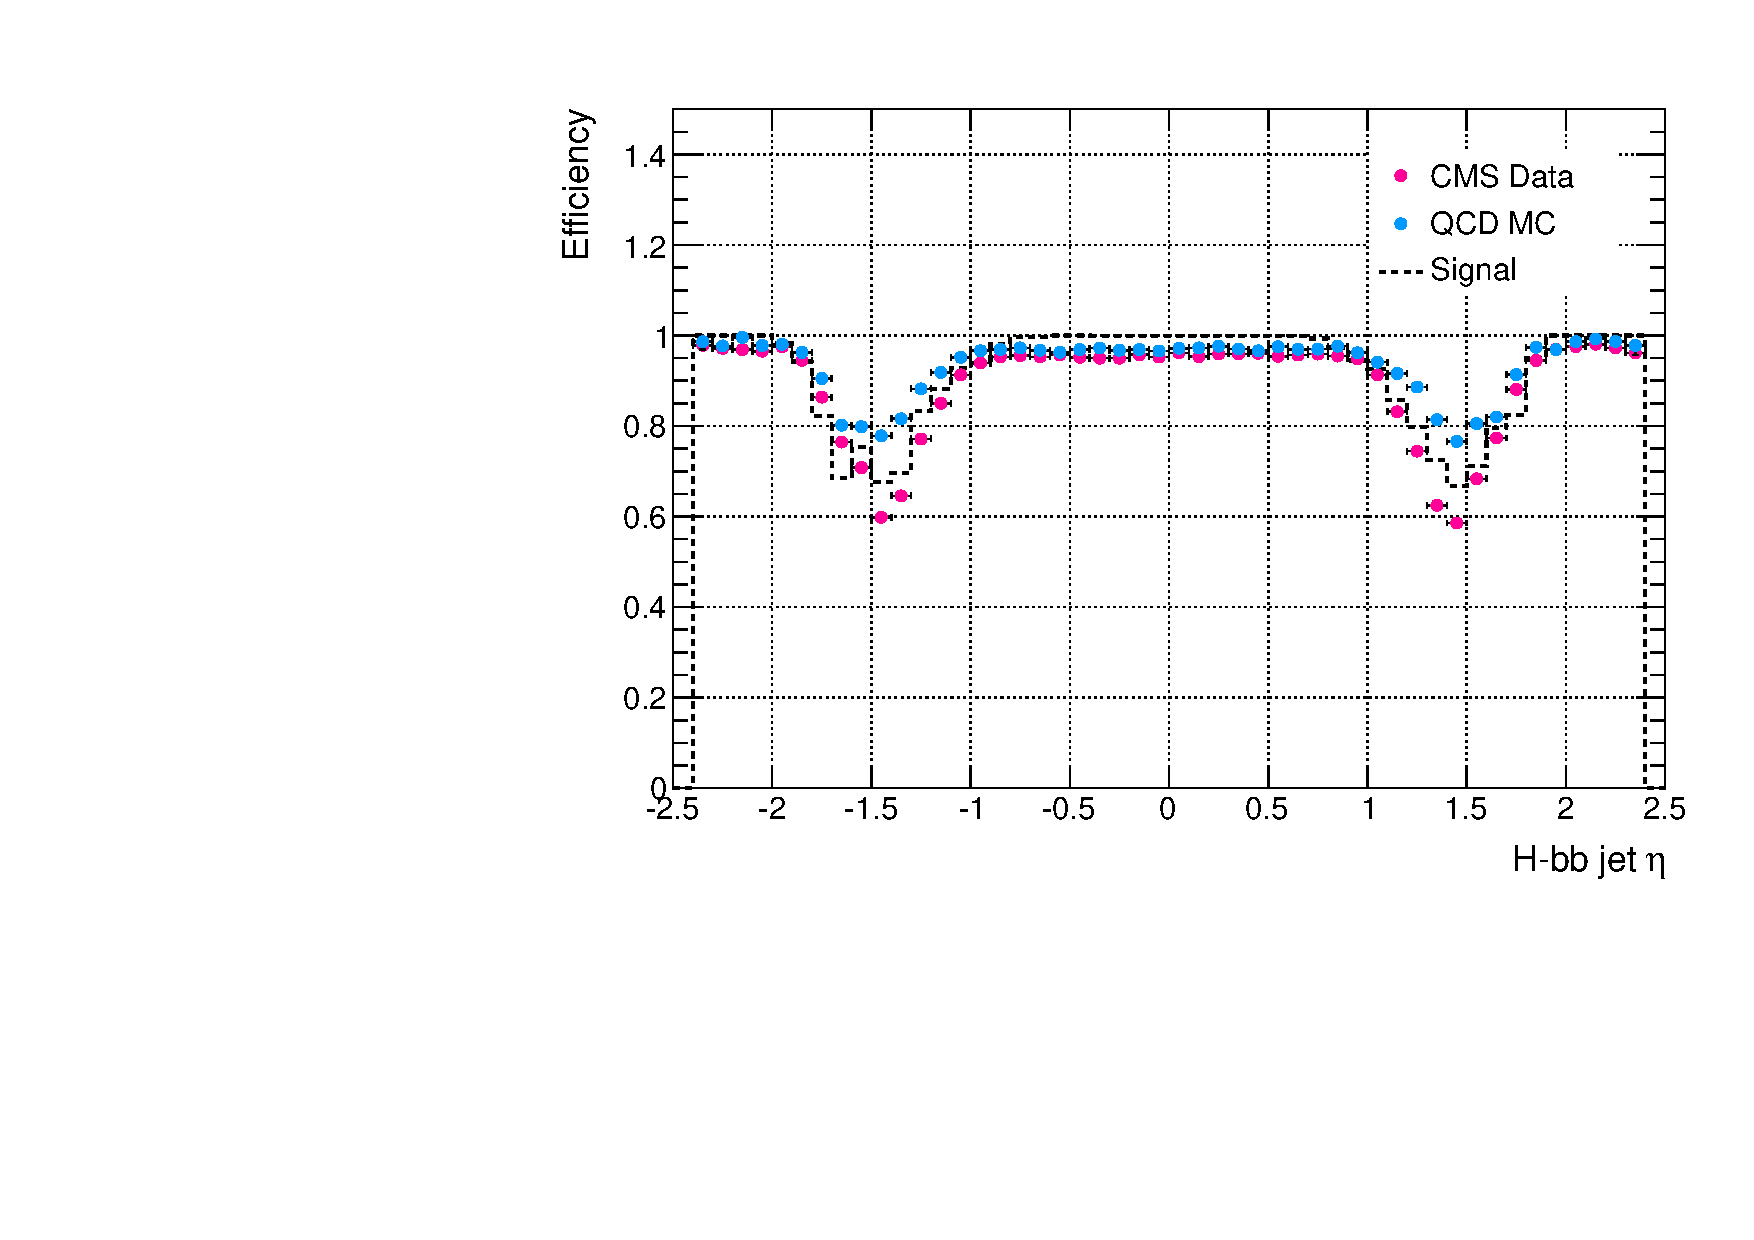
\includegraphics[width=0.45\textwidth]{Appendix/Figures/eff-eta-tobtecfilter.pdf}}
\subfigure[]{\label{fig:eff-filters-eta_b}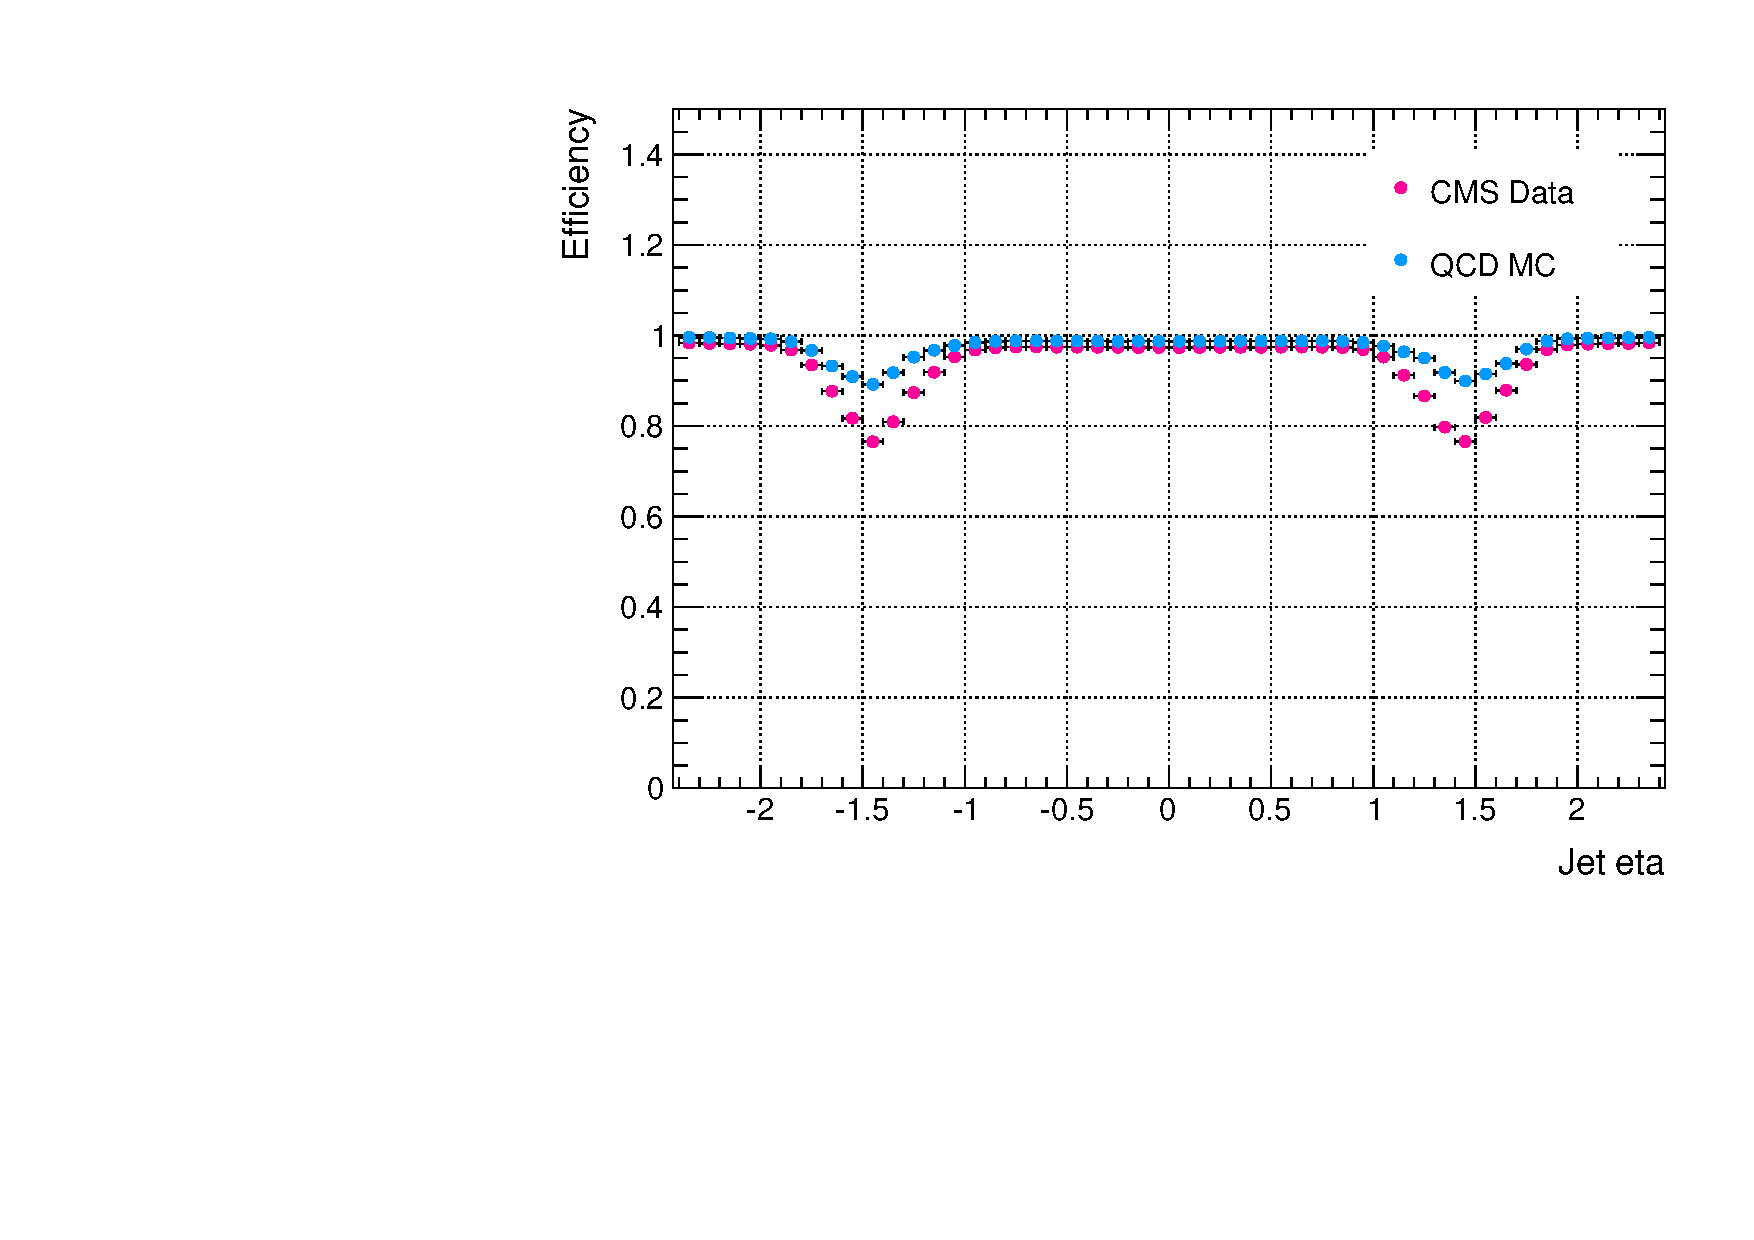
\includegraphics[width=0.45\textwidth]{Appendix/Figures/eff-eta-tobtecfilter-nobtag.pdf}}
\caption{Efficiency of the tracking noise filter as a function of the leading-jet \pt for data, and simulated signal and QCD background.
(a) The leading jet is required to be b tagged with the combined b-tagging algorithm used in the main analysis. (b) The b-tagging requirements for the leading jet are removed.}
\label{fig:eff-filters-eta}
\end{figure}

%\begin{table*}[thb]
%\caption{
%Summary of 8 TeV collision data used to study the efficiencies of the filters in data. The certification file used for these data is
%\texttt{Cert\_190456-208686\_8TeV\_22Jan2013ReReco\_Collisions12\_JSON.txt}.
%}
%\label{data-dijet}
%\vspace*{\medskipamount}
%\begin{center}
%\small
%\begin{tabular}{|l|}
%\hline
%\textbf{Dataset}\\
%\hline
%/Jet/Run2012A-22Jan2013-v1/AOD\\
%/JetHT/Run2012B-22Jan2013-v1/AOD\\
%/JetHT/Run2012C-22Jan2013-v1/AOD\\
%/JetHT/Run2012D-22Jan2013-v1/AOD\\
%\hline
%\end{tabular}
%\end{center}
%\end{table*}

%\begin{table*}[thb]
%\caption{
%Summary of the samples used to study the efficiencies of the two filters in simulation.
%}
%\label{mc-bkg-dijet}
%\vspace*{\medskipamount}
%\begin{center}
%\small
%\begin{tabular}{|l|}
%\hline
%\textbf{Sample}\\
%\hline
%/QCD\_HT-250To500\_TuneZ2star\_8TeV-madgraph-pythia6/\\
%Summer12\_DR53X-PU\_S10\_START53\_V7A-v1/AODSIM\\
%\\
%/QCD\_HT-500To1000\_TuneZ2star\_8TeV-madgraph-pythia6/\\
%Summer12\_DR53X-PU\_S10\_START53\_V7A-v1/AODSIM\\
%\\
%/QCD\_HT-1000ToInf\_TuneZ2star\_8TeV-madgraph-pythia6/\\
%Summer12\_DR53X-PU\_S10\_START53\_V7A-v1/AODSIM\\
%\hline
%\end{tabular}
%\end{center}
%\end{table*}